%Summary here
The system evaluation complements the system implementation by measuring the performance of the developed solution, answering RQ2. This evaluation process will be carried out following a sequential approach.

This section details the method and the principles that will be used to carry out the system evaluation process, measuring the performance (throughput, measured in rows/second) of reading and writing on Delta Lake or Apache Hudi while on \gls{HopsFS} of Spark-based and Rust-based pipelines. 

\subsection{Evaluation Process}
The research process will follow a sequential approach described in Figure \ref{fig:DevProcessRQ2}.

The first activity will consist of defining the research objectives for this quantitative system evaluation, then based on these objectives the benchmarks will be defined. Using the code implementation (D1), the benchmarks will be carried out generating a first set of raw data. This data will be modified according to the specified metric (throughput measured in rows/second), enabling the last step of this process: the results visualization. 

Each step of this process is related to one of the goals (G5-G8) associated to the RQ2 in Section \ref{sec:goals}. This process will produce two final deliverables which are the experiments results (D2), complete of data visualization and the results analysis (D3-partial).

\begin{figure}[!ht]
    \begin{center}
      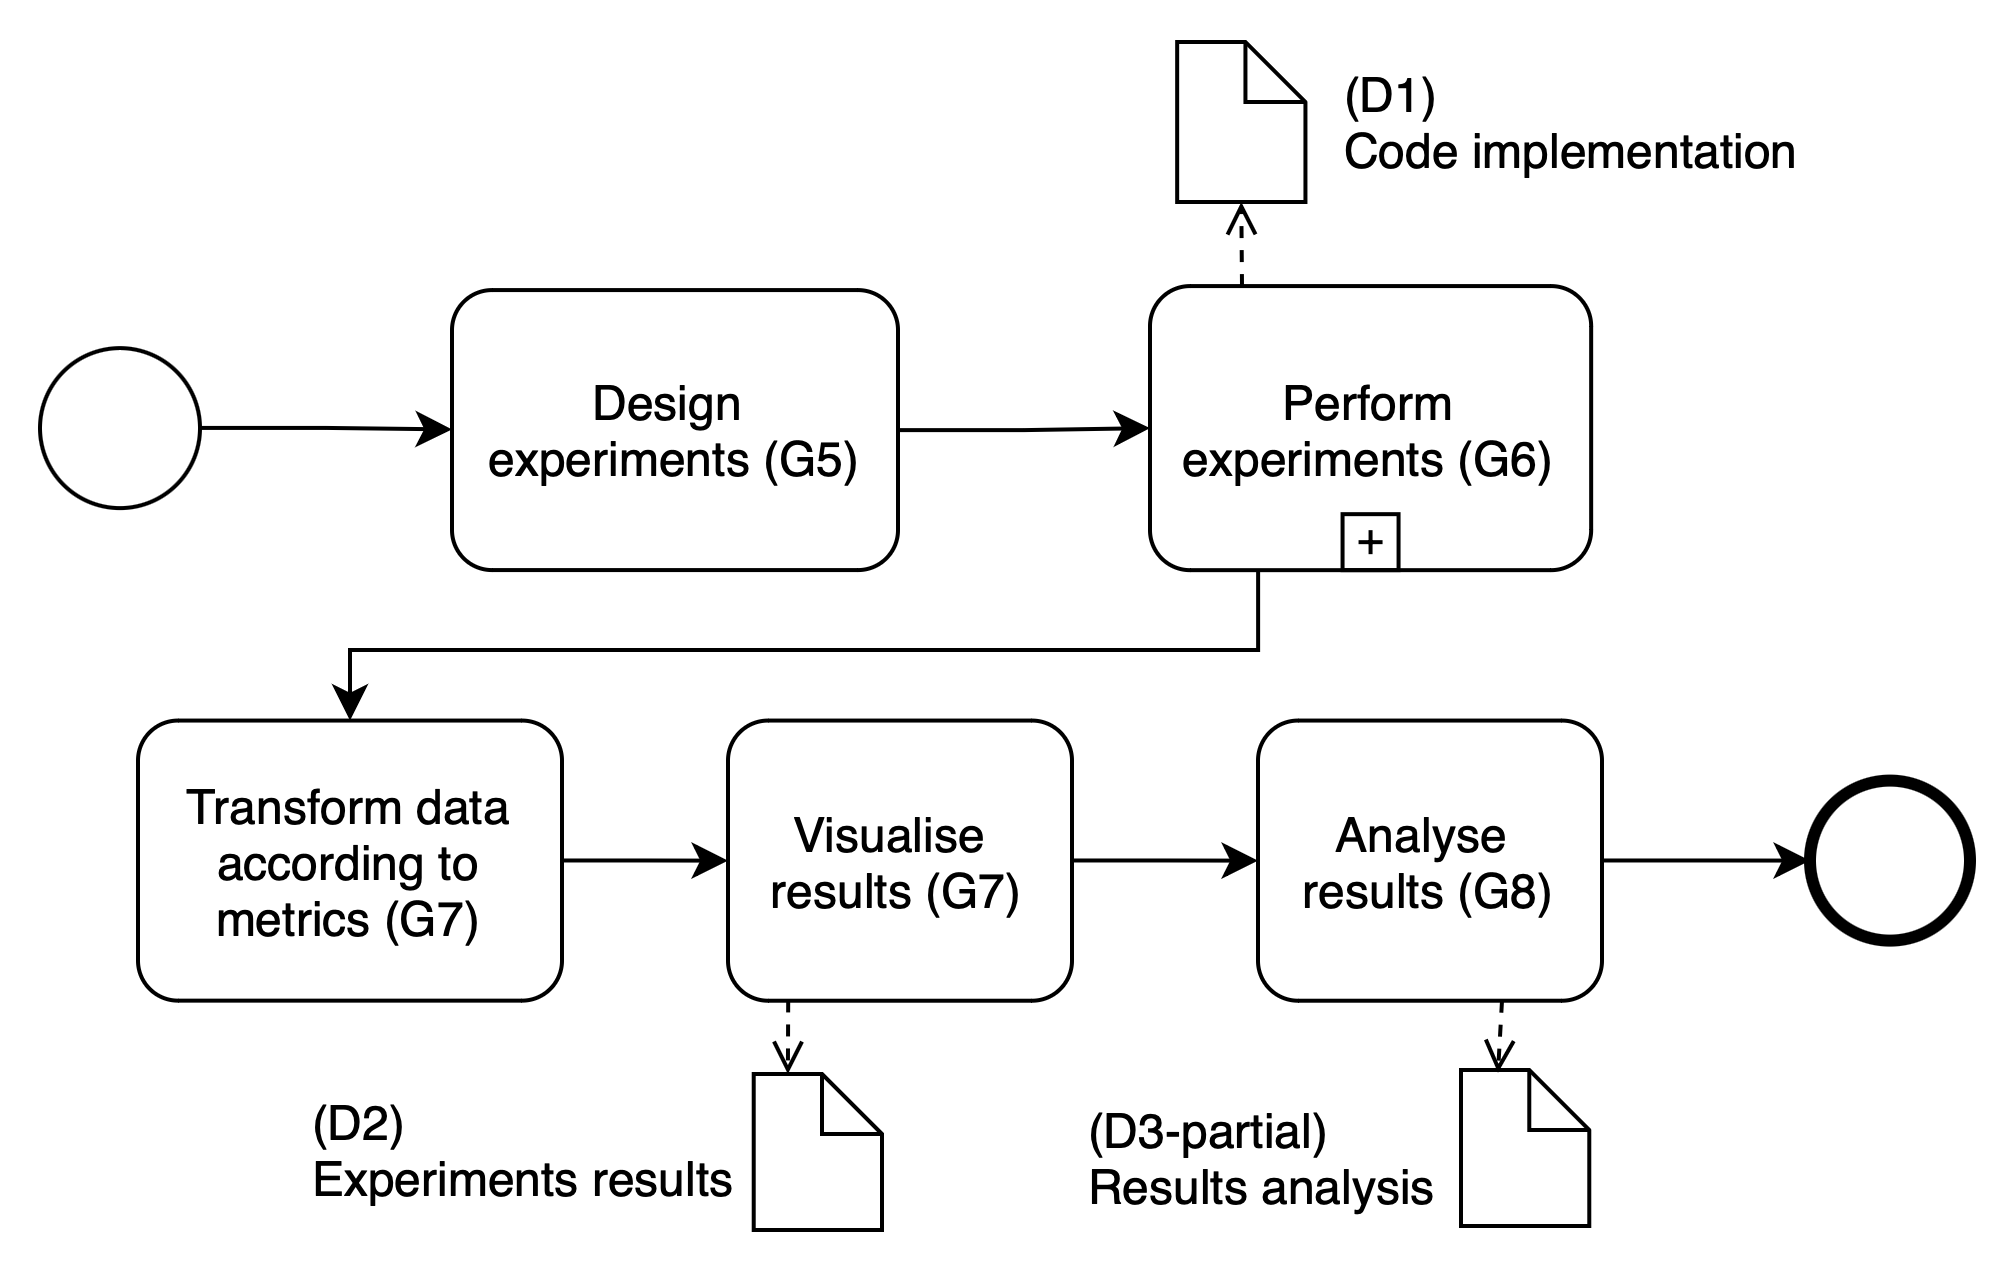
\includegraphics[width=\textwidth]{figures/3-method/research_process_rq2.png}
    \caption{\gls{BPMN} diagram of the System evaluation process answering to RQ2. Each activity is associated to a specific Goal (\gls{G}). The process produces two deliverables (\gls{D}), the experiments results (D2) and a results analysis (D3-partial).}
    \label{fig:DevProcessRQ2}
    \end{center}
\end{figure}

\subsection{Research Paradigm}
The research paradigm consists of a quantitative analysis based on repeated runs on the implemented system. The results of the benchmarks are then analyzed performing a visual comparative approach.

\subsection{Dataset}
\label{subsec:dataset}

The dataset that will be used to perform the read and write operations is the TCP-H \cite{TPCHHomepage}. This dataset is used at it provides a recognized standard for data storage systems \cite{TPC_benchmarks_2000}. Any part of the dataset can be generated using TPC-H data generation tool \cite{TPCCurrentSpecs}.

The TCP-H dataset contains eight tables, of these two, SUPPLIER and LINEITEM, were selected for the following reasons. The two tables are respectively the smallest (10000 rows) and largest (6000000 rows) table which size (number of rows) depends on the \gls{SF}. The \gls{SF} can be varied to obtain tables of different sizes (number of rows), allowing to a progressive change in the table size (number of rows). 

The SUPPLIER table has seven columns, while the LINEITEM table has sixteen. This influences the average size of memory each row occupies. This means that the metric selected (throughput, measured in rows/second) cannot be used to compare results across different tables. This is the reason why the comparative evaluation only considers different configurations on the same table. 

For this project five table variations were used to benchmark the code solution as D1. \gls{SF} was varied to obtain a table at each significate figure, from 10000 rows to 60000000 rows. These are the tables:
\begin{enumerate}
    \item \textit{supplier\_sf1}: size = 10000 rows
    \item \textit{supplier\_sf10}: size = 100000 rows
    \item \textit{supplier\_sf100}: size = 1000000 rows
    \item \textit{lineitem\_sf1}: size = 60000000 rows
    \item \textit{lineitem\_sf10}: size = 60000000 rows
\end{enumerate}

\subsection{Experimental Design}
% Description of which benchmarks will be performed and how. Here it needs to be explained the environment where the benchmarks will be run (Snurran), which tests are run and why in this particular way.
%
% Talk about the selection of the questions: How do the performances vary if: (1) the new implemented pipeline is used vs. the old pipeline. (2) a simple localFilesystem implementation is used vs. writing on \gls{HopsFS} (3) varying the CPU configuration (4) we have different table sizes. 

The experiments aim is to highlight the differences between the newly implemented system based on the delta-rs library, and the legacy Spark-based system. To isolate the benefit of using delta-rs over Spark and provide a baseline, three different testing pipelines were designed:
\begin{enumerate}
    \item \textbf{delta-rs - \glsentryshort{HopsFS}}: the system implemented in Chapter \ref{ch:implementation}. It is composed of a Rust pipeline with Python bindings, that enables performing operations (i.e. reading, writing) on Delta Lake tables. This pipeline writes on \gls{HopsFS}.
    \item \textbf{delta-rs - \glsentryshort{LocalFS}}: this pipeline uses the same library as the system implemented, but saves data on the \gls{LocalFS}. This provides a comparison within the delta-rs library, isolating the impact on performance caused by writing on \gls{HopsFS}, a distributed file system.
    \item \textbf{Legacy Spark pipeline}: this pipeline uses the Hopsworks Feature Store to write data on Hudi tables. This system makes use of a pipeline based on Kafka, and Spark to write data on the Hudi tables, saved on \gls{HopsFS}. 
\end{enumerate}

Furthermore, the experiments will verify how performances of three system will change based on the \gls{CPU} resources provided (namely 1 core, 2 cores, 4 cores, 8 cores). Each time the testing environment will be modified accordingly, creating a new \gls{VM} where the experiments will run with increasingly more resources. These \gls{CPU} configurations were chosen together with the industrial supervisor, according to the typical Hopsworks use case.

The data used for experiments, as described in Section \ref{subsec:dataset}, will come from two different tables. These are modified according to a \gls{SF}, for a total of five times.

In conclusion the experiments conducted will be a total of 3 (pipelines) times 4 (\gls{CPU} configurations) times 5 (tables) times 2 (read and write operations), i.e. 120 experiments, performed 50 times each to create statistically significant results.

\subsection{Experimental environment}
% Describe Snurran
The experimental environment consists of a physical machine in Hopsworks' offices, virtualized for enabling remote shared development. The \gls{CPU} details of the machine are present in Listing \ref{lst:cpu_snurran}, noting that only eight cores at maximum were accessed during the experiments.

The machine mounts about 5.4 TBs of \gls{SSD} memory. This allows the machine to have fast read and write speed, 2.7 GB/s and 1.9 GB/s respectively (measured with a simple \textit{dd} bash command).

\begin{lstlisting}[language=bash, caption={Output of a \textit{lscpu} bash command on the test environment.}, label={lst:cpu_snurran}, frame=tb]
Architecture:            x86_64
  CPU op-mode(s):        32-bit, 64-bit
  Address sizes:         48 bits physical, 
                         48 bits virtual
  Byte Order:            Little Endian
CPU(s):                  32
  On-line CPU(s) list:   0-31
Vendor ID:               AuthenticAMD
  Model name:            AMD Ryzen Threadripper 
                         PRO 5955WX 16-Cores
    CPU family:          25
    Model:               8
    Thread(s) per core:  2
    Core(s) per socket:  16
    Socket(s):           1
    Stepping:            2
    Frequency boost:     enabled
    CPU max MHz:         7031.2500
    CPU min MHz:         1800.0000
    BogoMIPS:            7985.56
Virtualization features: 
  Virtualization:        AMD-V
Caches (sum of all):     
  L1d:                   512 KiB (16 instances)
  L1i:                   512 KiB (16 instances)
  L2:                    8 MiB (16 instances)
  L3:                    64 MiB (2 instances)
\end{lstlisting}
\FloatBarrier

\subsection{Assessing Reliability and Validity}
% Here explain how the readability and validity of the collected data was addressed. Mainly here the bootstrapping method need to be explained and how it achieves getting a CI without making assumption on the data distribution

Results are significant according to their reliability and validity. In this project work, to ensure the reliability of the experiments results on the system performance, each experiment will be performed fifty times. This number was agreed as a balance between consistency and the limited resources available (in terms of time and computing resources).

Probably due to the complex nature of the pipeline tested, the data distribution of results could vary from one experiment to the other. This hampers the possibility of comparing results, greatly impacting on the relevance of the results analysis. To restore the validity of the data collected a bootstrapping technique will be used. Data will be resampled with substitution a thousand times, then calculating an average and a confidence interval for each experiment. This will benefit the accuracy of the results presented.